
\begin{figure*}[ht!]
	\begin{center}
		%    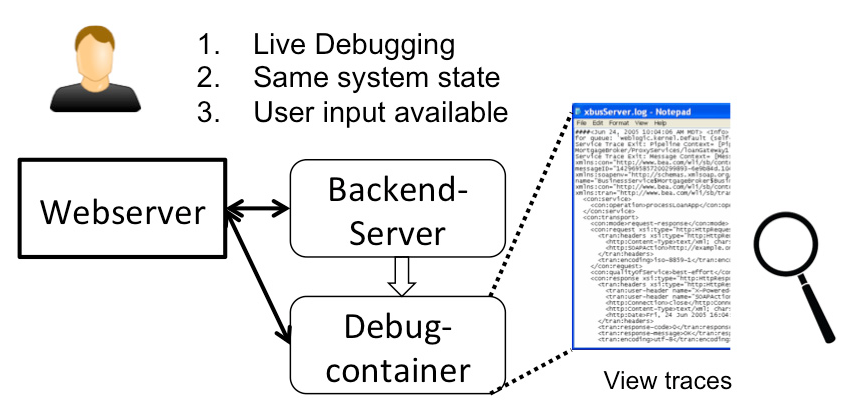
\includegraphics[width=0.7\textwidth]{figs/motivation.eps}
		\includegraphics[width=0.9\textwidth]{figs/workflow3.pdf}
		\caption{Workflow of \parikshan in a live multi-tier production system with several interacting services. When the administrator of the system observes errors in two of it's tiers, he can create a sandboxed clone of these tiers and observe/debug them in a sandbox environment without impacting the actual production system.}
		\label{fig:motivation}
	\end{center}
\end{figure*}



\section{Background}
\label{sec:background}

In this section, we give a short description of the design of live debugging and our \parikshan framework to facilitate the exposition of the ideas in this paper. 
%A detailed explanation of the complete design of the paper can be found in ~\cite{parikshan}.

\subsection{The case for Live Debugging}
\label{sec:case}

Figure \ref{fig:motivation}, shows a high level overview of ``live debugging'' in action. 
The figure shows a live production system with multiple services. 
The system is maintained by an operator, who can observe the health of the system using light-weight monitoring, which is part of the deployed system. 
In the interest of application performance, production system monitoring is usually limited to system resource usage, application usage statistics, transaction logs, and error logs.

Let us assume that at a certain time in the execution of the system, the operator observes unusual memory usage in the glassfish application server, and some error logs being generated in the nginx webserver. 
Typically, trouble tickets are generated for such problems, and they are debugged offline.
However, the operator can now use \parikshan to fork off clones of the nginx and glassfish containers as \textbf{nginx-debug} and \textbf{glassfish-debug}.
Network duplication mechanisms ensure that the debug-containers receive the same inputs as the production, and the production containers continue to provide service without interruption.
This seperation of production and debug environments allows the operator to use dynamic instrumentation tools to do deeper diagnosis without fearing any problems in the user-facing operations.
Since the system has been cloned from the original potentially ``buggy'' production container, it will also exhibit the same memory leaks/or logical errors.
Additionally, \parikshan can focus on the ``buggy'' parts of the system, without needing to replicate the entire system in a test-cluster. This process will greatly reduce the time to bug resolution, and allow real-time bug diagnosis capability.

\subsection{Design Overiview}
\label{sec:design}

Our system called \parikshan, is composed of three modules:\\

%\begin{itemize}
%	\item 

\noindent \subsubsection{Clone Manager}
The clone-manager manages ``live cloning'' between the production and debug containers.
``Live Cloning'' refers to the process of copying a running virtual machine, or container from one server to another, without disconnecting any client or process running within the service.
This generates two containers, a production container which serves the actual user requests, and a debug-container which gets the same input as the production but is maintained only for debugging purposes.
The ``live'' part in the cloning process means that cloning has a very small suspend time and the service is kept active while cloning. \\

	
	\begin{figure}[ht]
		\begin{centering}
			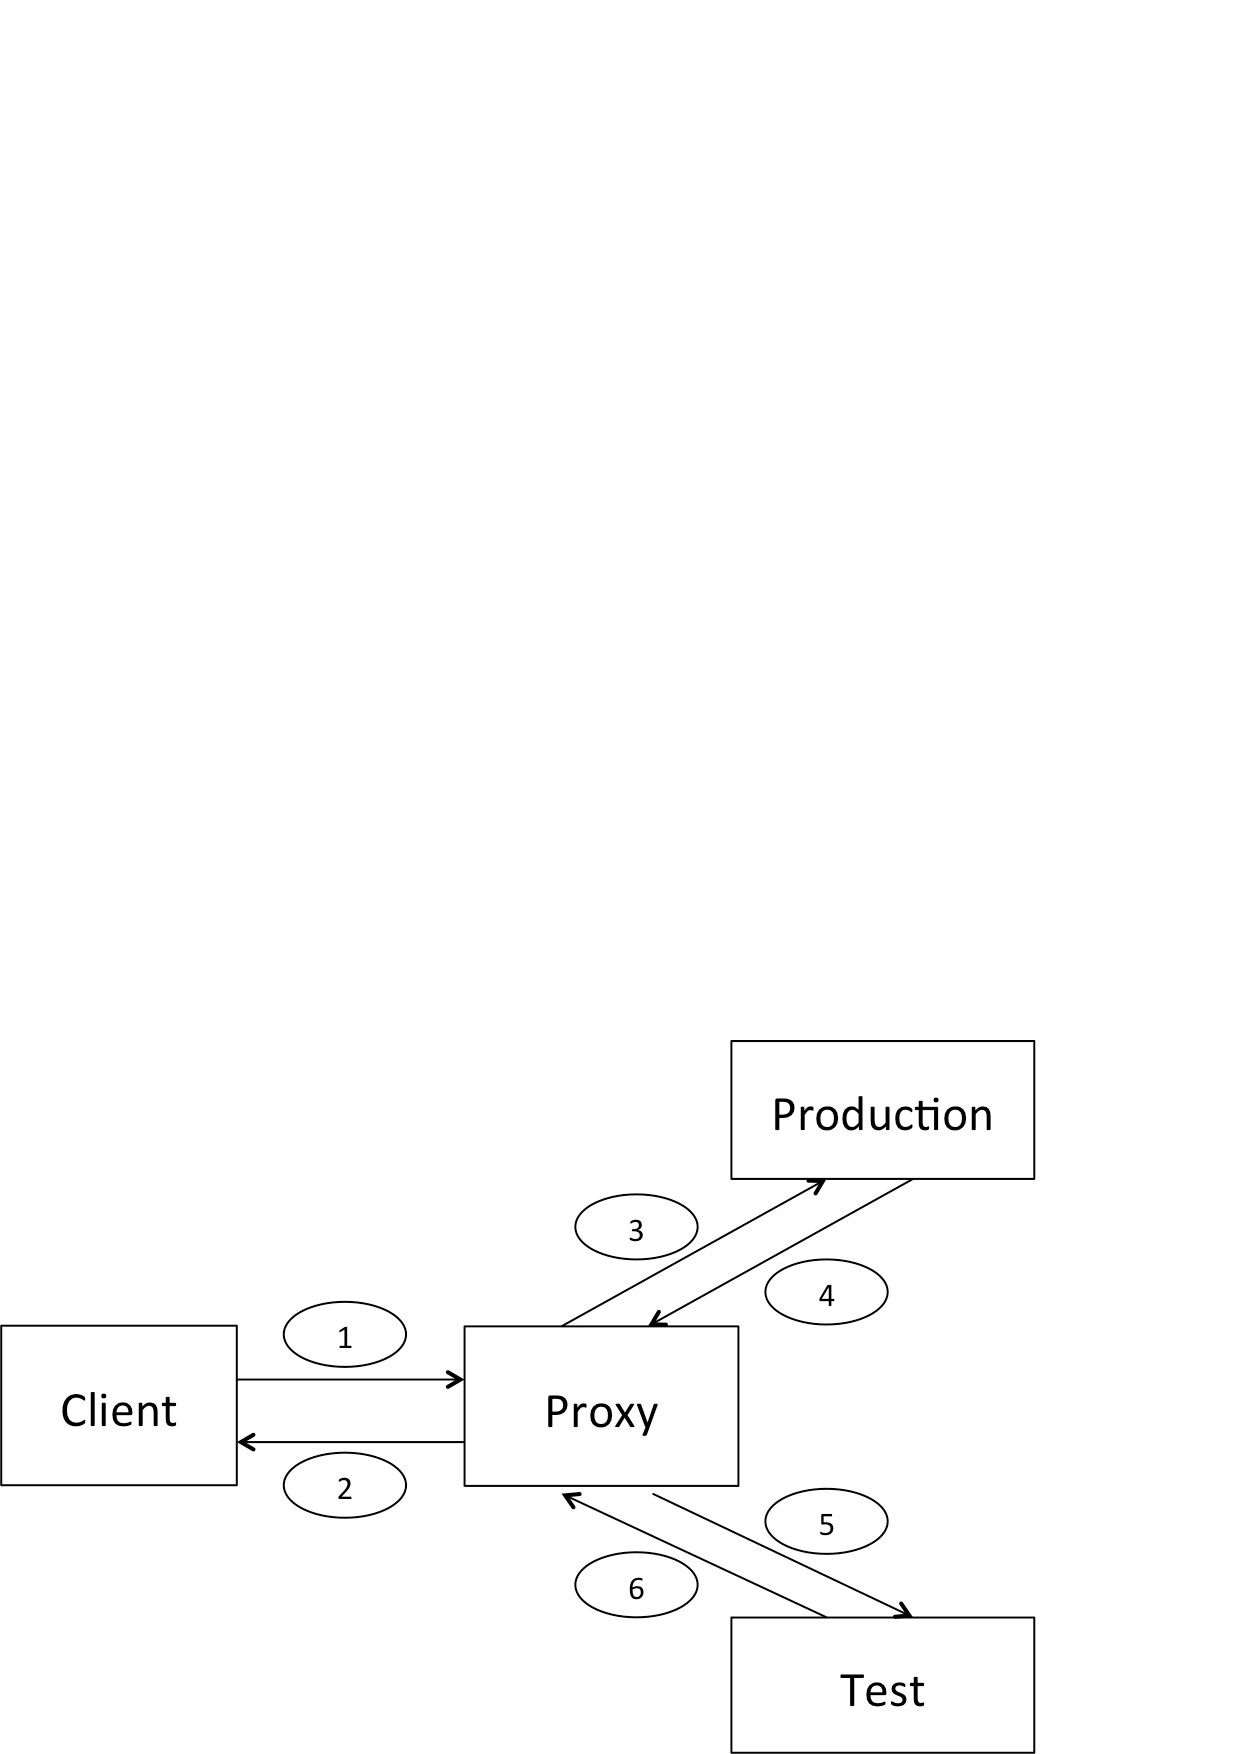
\includegraphics[width=0.7\textwidth]{figs/network_dup.pdf}
			%    \captionsetup{justification=centering}
			\caption{Description of the Network Duplicator: Thread 1 executes steps [1,3], Thread 2 executes [2,4], Thread 3 executes [5], and Thread 4 executes [6]}
			\label{fig:duplicator}
		\end{centering}
	\end{figure}

%\item 
\noindent \subsubsection{Network Duplicator} 
The network duplicator manages communication from the client to both the production container and the debug container.
The basic design is based on a customized TCP level proxy, which duplicates network traffic to both these containers.
As shown in figure~\ref{fig:duplicator}, the duplicator uses an asynchronous packet forwarding model, with 4 threads for each incoming connections.
Thread T1 forwards packets from client to proxy (link 1), and from proxy to production container(link 2). It then uses a non-blocking send to foward packets to an internal pipe buffer shared between thread T1, thread T3. Thread T3, then reads from this piped buffer and sends traffic forward to the debug-container. 
Similarly Thread T2, receives packets from production container, and forwards them to the client, while thread T4, receives packets from debug container and drop them. 

The advantage of this strategy is that any slowdown in the debug-container will not impact the production container.
However, a side-effect is that if the speed of the debug-container is too slow compared to the production container, it may lead to a buffer overflow. 
We call the time taken by a connection before it overflows, it's \textbf{debugging window}.
We assume that both the production and debug containers are identical for the purposes of debugging as long as we do not have an overflow. \\

\begin{figure}[ht]
	\begin{center}
		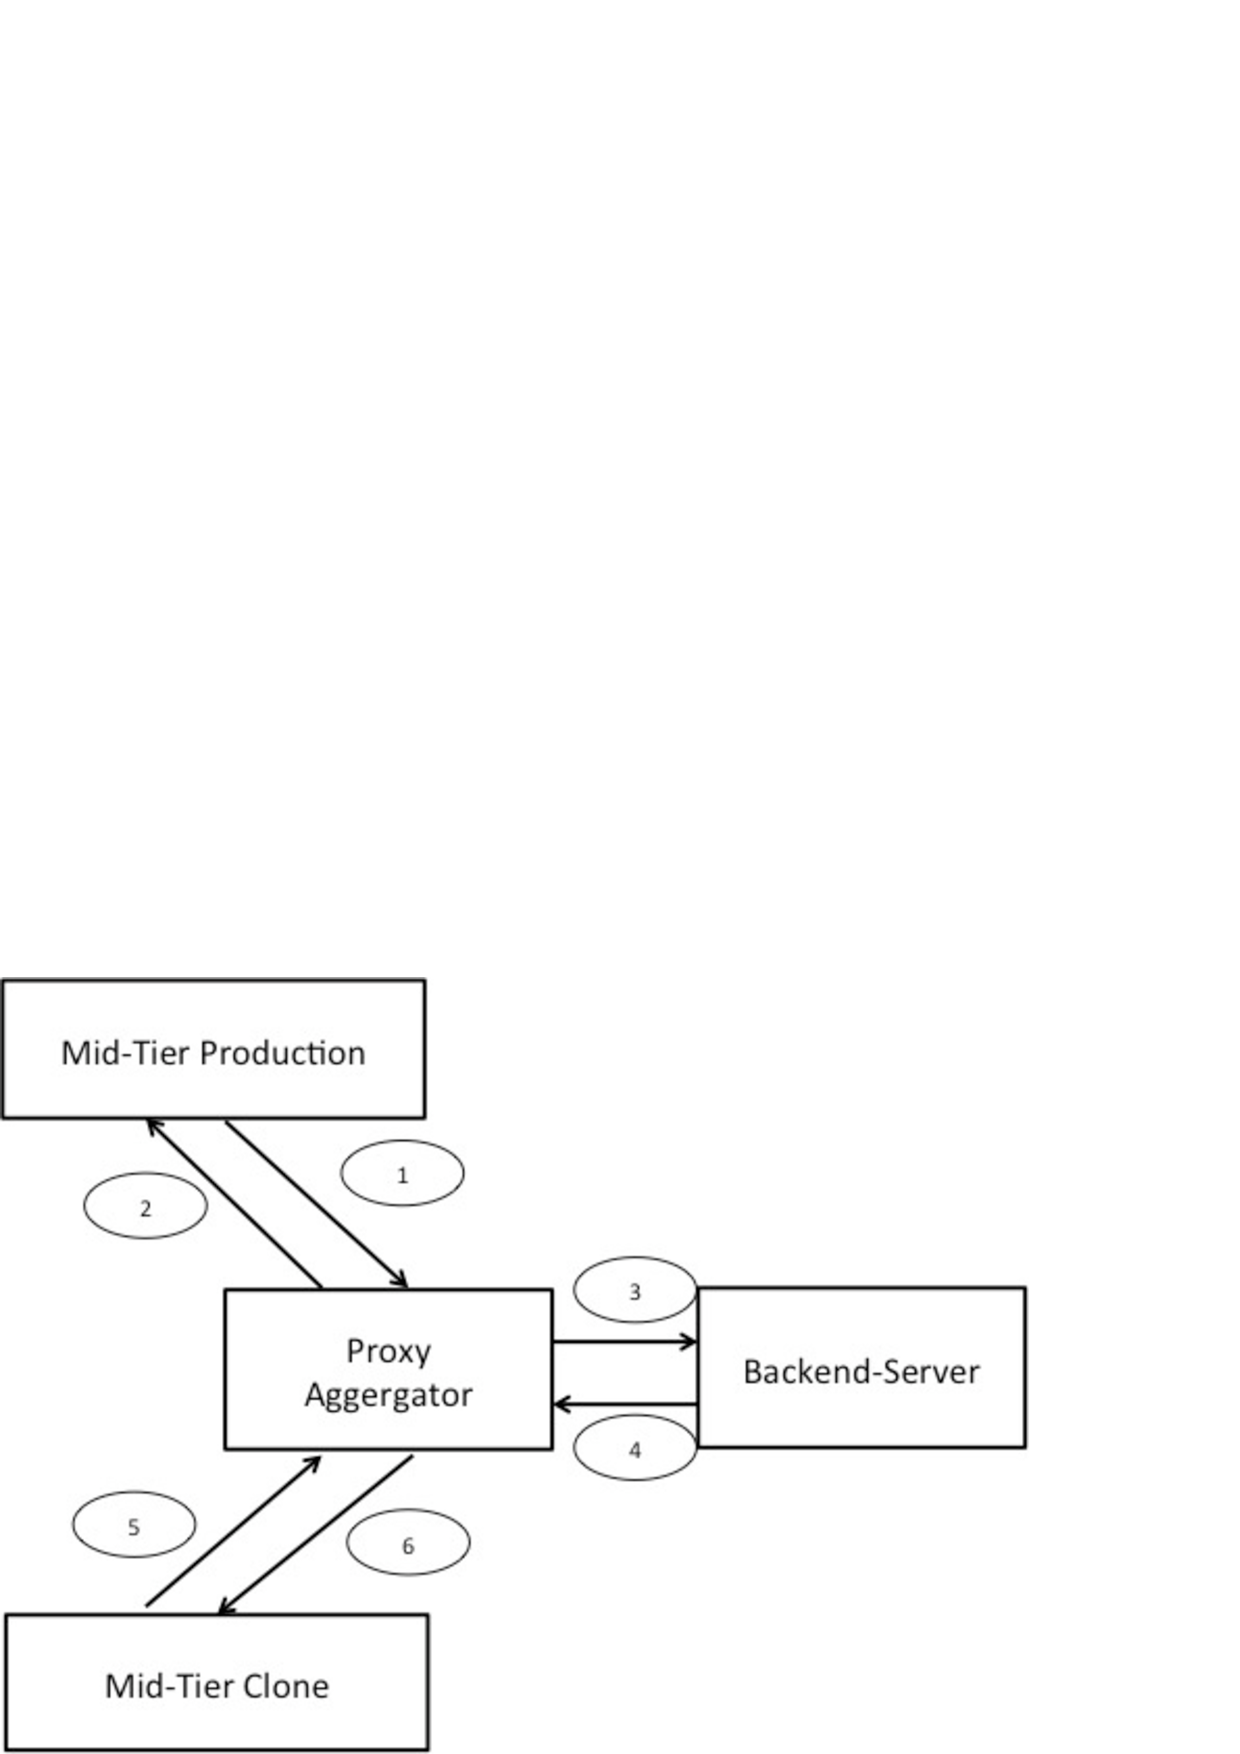
\includegraphics[width=0.7\textwidth]{figs/aggregator.pdf}
		%    \captionsetup{justification=centering}
		\caption{Description of the Network Aggregator. Thread 1 executes step [1,3], Thread 2 executes [2,4], and Thread 3 executes [5], and Thread 4 executes [6]}
		\label{fig:aggregator}
	\end{center}
\end{figure}

\noindent \subsubsection{Network Aggregator} 
The ``proxy aggregator'' module stubs the requests from a duplicate debug container by replaying the responses sent to the production container, to the debug-container.
As well as dropping all packets sent from it to upstream servers.

As shown in  Fig~\ref{fig:aggregator}, when an incoming request comes to the aggregator, it first checks if the connection is from the production container or debug container. 
In case of the production container (link 1), the aggregator forwards the connection to the backend (link 3), responses from the backend are sent to the aggregator (link 4), and then forwarded to the production container (link 2) and simultaneously saved in an internal queue.
The aggregator creates an in-memory persistent inter-process FIFO queue for each connection where the responses for each of these connections are stored.
When the corresponding connection from the duplicate debug container connects to the proxy (link 5); all packets being sent are quietly dropped. 
The aggregator then uses the queue to send replies to the debug-container (link 6).
In a way this is a streaming online record-and-replay, where we are recording the data in our buffer.
We assume that the production and the debug container are in the same state, and are sending the same requests. 
Hence, sending the corresponding responses from the FIFO stack instead of the backend ensures: (a) all communications to and from the debug container are isolated from the rest of the network, (b) the debug container gets a logical response for all it's outgoing requests.

In this design we assume that the order of incoming connections remains largely the same.
We use a fuzzy checking mechanism using the hash value of the data being sent to correlate the connections. 
Each queue has a short wait time to check against incoming connections, this allows us to match slightly out of order connections.
In case a connection cannot be correlated, we send a TCP\_FIN, to close the connection, and inform the debugger.

\par
\noindent \subsubsection{Debug Window} 
%At the time of the live cloning, the testing container has an identical status and receives the same input as the production container. 
%Hence, any test-cases run in the testing container, should faithfully represent the status of the production container.
%However, an obvious down-side to any debugging/testing is that it will add an overhead on the performance of the test-container as compared to the production environment.
%This would mean that the execution of requests in the test-container will lag behind the production container. 
%To avoid this slowdown impacting the actual production container, 
%\noindent
The network duplicator forwards traffic using an unblocking send to a separate thread which manages communication to the debug-container. 
This thread has an internal buffer, where all incoming requests are queued, and subsequently forwarded to the debug-container. 
The incoming request rate to the buffer is dependent on how fast the production container manages the requests (i.e. the production container is the rate-limiter).
Whereas the outgoing rate from the buffer is dependent on how fast the debug-container processes the requests.
Because of instrumentation overhead in the debug-container, the outgoing rate is likely to be less than the production container.
The time period till buffer overflow happens is called the \emph{debug-window}.
This depends on the size of the buffer, the incoming request rate, and the overhead induced in the debug-container. 
For the duration of the debugging-window, we assume that the debug-container faithfully represents the production container. 
Once the buffer has overflown, the production container may need to be cloned again to ensure it has the same state.

%\noindent
The debug window size also depends on the application behavior, in particular how it launches TCP connections. 
\parikshan generates a pipe for each TCP connect call, and the number of pipes are limited to the maximum number of connections allowed in the application.
Hence, buffer overflows happens only if the requests being sent in the same connection overflow the queue.
For webservers, and application servers, the debugging window size is generally not a problem, as each request is a new ``connection'', hence the proxy is able to tolerate significant slowdowns.
Database servers, and other session based services usually have small request sizes, but multiple requests can be sent in one session which is initiated by a user. 
In such cases, the amount of calls in a single session can eventually have a cumulative effect to cause overflows.
Photosharing, file sharing and other datasharing services transfer a lot of data in a single burst over each TCP connection. 
These protocols will have an overflow relatively sooner, and will be able to tolerate only small amounts of slowdown. 

To further increase the \emph{debug window}, we propose load balancing debugging across multiple debug-containers, which can each get a duplicate copy of the incoming data. 
This would mean that there are multiple threads handling the incoming connection, one for the production container, and one for each of the debug containers.
We believe that such a strategy would significantly reduce the chance of a buffer overflow in cases where the debug-container is significantly slower.
We evaluate debug-window overflows in section~\ref{sec:timewindowPerformance}.